\documentclass[UTF8,a4paper]{ctexart}
\usepackage[margin=1in]{geometry}
\usepackage{fancyhdr,hyperref,amsmath,float,graphicx,color}
\pagestyle{fancy}
\hypersetup{hidelinks}

\lhead{\bfseries \leftmark}
\chead{}
\rhead{SCUT}
\lfoot{\url{https://github.com/285571052}}
\cfoot{qhy}
\rfoot{\thepage}
\setlength{\headheight}{13pt}
\renewcommand{\headrulewidth}{0.4pt}
\renewcommand{\footrulewidth}{0.4pt}

\setlength{\parindent}{0pt}
\newcommand{\spaceline}{\vspace{\baselineskip}}

\author{ qhy }
\date{\today}
\title{编译原理}

\begin{document}
  \maketitle
  \tableofcontents
  \newpage

  \section{介绍}
  2017-9-5:第一节课主要简单介绍的mac地址,ip以及协议相关内容。

  \section{数字调制和复用}
  \textbf{波特率:}每秒信号变化的次数。
  \[C = B \times \log_2 n\]

  \spaceline
  $\left \{ \begin{array}{l}
  \text{基带传输:使用高低调位为标准描述0/1两个信号}\\
  \text{通带传输:使用振幅,频率,相位等为标准描述}
  \end{array} \right .$

  基带传输的几个例子:???
  通带传输的3个例子:???

  信号星座?\\
  通带传输3种情况的综合应用:使用不同相位、波长表示不用的信号,这样接受一个符号,这个符号能表示的范围就变大,从而减少传输的时间。\\
  比如每次接受一个波形,能可能表示4个情况,那么这个波形就能表示两个位(00,01,10,11)的一种

  例子????

  \textbf{复用技术:}多个用户使用同一个通道。\\
  前面相位、波长用来表示数字,而频率和其他冗余信息则主要用于复用技术方面。

  复用技术主要有以下几种类型:
  \begin{itemize}
    \item 频分多路复用(FDM)\\
    不同频率直接迭代,最终经过滤波器分开
    \item 正交FDM\\
    普通的FDM每个频率段之间是不交的,而正交FDM有相交部分,但是也能区分开来
    \item 时分多路复用\\
    时间上共享,一个接一个使用
    \item 统计时分多路复用\\
    时分多路复用的话,是每个用户一次分配到使用时间,不管有没用到,而统计时分多路复用则是没有用到就不分配时间
    \item 码分多路复用\\
    每个用户拥有一个唯一的码片,每个码片相互正交(主要用于3G网络)\\
    比如,传送4位信号,里面能包含3个用户发送的信息情况等。
  \end{itemize}

  冲突:同时发送数据,引起冲突

  怎么防止冲突?减小冲突域

  调制解调器的任务是把数字信号转换成模拟信号

  TCM:每次采样中,有一位用于纠错

  电话线拨号上网(不经过猫)的56K是怎么计算出来的?

\section{第四章}
\textbf{ALOHA协议}:想什么时候发送数据帧就什么时候发送

\textbf{分槽ALOHA协议:}
\begin{itemize}
  \item 时间分槽,只有在时间槽开始的时候才能发送数据帧
  \item 一个时间槽只有一个帧,那么这一帧一定能成功发送
  \item 多个帧发送,那么均发送失败,这个时间槽作废
  \item 时间槽一般取帧时
\end{itemize}

\textbf{统计规律:}每个时间帧发送k个数据的帧数满足泊松分布
$P_r[k] = \frac{G^kE^{-G}}{k!}$
其中,G表示,帧时T内,信道内的帧数(包括重发的)

\textbf{吞吐率S:}在发送时间T内成功发送的平均帧数

\textbf{信道利用率:}T为单位时间的时候的吞吐率

根据定义有:$S = GP_0$,其中$P_0$表示一帧发送成功的概率。那么问题是,$P_0$怎么求?

对于ALOHA协议,当一个发送端想要发送数据的时候,它想要发送成功,就要求发送的时间段内没有其他数据帧发送。
而发送端所占的时间,至少会有两个帧时是处于危险期(可能冲突),因此需要两个帧时都没有数据帧,根据前面的分布规律\\
$P_0 = (Pr[0])^2 = e^{-2G}$

而对于分槽的ALOHA协议,只要没有其他人抢占帧时,那么就一定能发送成功,因而只需要考虑一个帧时内没有数据帧即可,因此\\
$P_0 = Pr[0] = e^{-G}$

$ALOHA$协议的应用:
\begin{itemize}
  \item 电缆传送数据
  \item 基站之间发送数据
  \item 多个RFID与RFID读写器
\end{itemize}

\textbf{载波侦听多路访问协议:}先听后写\\
当一个站有数据要发送的时候,首先看线路上是否有其他线路发送数据
\begin{itemize}
  \item 坚持\\
  忙等,当信道忙的时候,一直等待监听,直到空闲
  \item 非坚持\\
  当信道忙的时候,先随机等待一段时间,再进行监听
  \item p-坚持\\
  前两种的这种,当信道空闲的时候,有p的概率发送,有1-p的概率继续等待随机时间(为了避免抢占信道时候的冲突)
\end{itemize}

这种协议,在信道忙的时候不会冲突,而当信道闲的时候,还是可能发生冲突
\begin{itemize}
  \item 第一种情况是,多个帧等待发送
  \item 第二种情况是,由于延迟问题,一个发送端抢占信道之后,另一端未能检测到继续发送而导致冲突
\end{itemize}
物理层上信号的传输:信号
有两类:
1. 模拟信号
2. 数字信号

信号在传输的过程中,接收方接受到的信号可能是衰减和变形的(失真)

截至频率fc,一般来说0~fc这一段频率,振幅在传输的过程中不会明显衰减

物理带宽:传输过程中振幅不会明显衰减的频率范围{这个频率是什么?}

数字带宽:单位时间内传输的信息的总量

物理带宽和数字带宽的关系是?

奈奎斯特定理:
在无噪声信道中,当带宽为B Hz(物理带宽),信号电平为V级,则最大传输速率(数字带宽)=$2Blog_2 V$ (bps,一秒钟信号变化的次数,物理带宽和波特率的关系?)
其中,V为信号的点评级数,在二进制中卫0、1两级

而物理带宽在信道确定的时候也跟着确定,因此要提高数字带宽,只能提高电平级数。

{这个公式怎么理解?最多2B次采样什么意思,V级别什么意思?2B是采样率/波特率,B Hz的最大采样率为2B Hz}

香浓定理

两道习题?

/****************/
传输介质
1. 铜线
	1. 同轴电缆
	2. 双绞线
		1. UDP.非屏蔽双绞线:成本低,尺寸小,易于安装,但易受敢逃,传输距离性能,收到绞距,10~100Mbps、最大传输距离100m(短)
		2. STP,屏蔽双绞线(4对线,每对线都有屏蔽层,最外面还有一层屏蔽层),成本高,安装不容易(最大距离100m,10~1000=Mbps,
		3. 网屏式双绞线,保留最外的屏蔽层
		除了屏蔽性能,其他是一样的

		双绞线的线序:568B,568A(直通线,两根头的线序相同,交叉线,线序相反)
	3. 电力线
2. 光纤
	3层,两层玻璃纤维,最外层为防护层,重量轻,损耗低,不受电磁辐射干扰,传输带宽大但昂贵易断
	原理:全反射,因而损耗低
	单模光纤:单一模式传输(平行入射),运行波长850~1300nm,纤芯细8~10um,激光产生但束光,高带宽,长距离
	多模光纤:多个模式同时传输(多个角度入射,只要大于临界角度,运行波长1310nm或1550n,纤芯粗50~62.5um,LED产生多束光。低带宽,短距离

	光纤连接:光纤连接器损失10~20%,机械拼接,特殊的套管加紧(10%),熔合几乎无损失

3. 无线电,卫星,激光

/***********************/
复用技术:让多个用户共享同一根信道
FMD:频分多路复用:将频谱分成若干段,每个用户占据一段来传输自己的信号

OFDM,正交FDM,相邻两个波之间可以重叠,

TDM:时分多路复用,用户分时轮流使用,

stdm:统计时分多路复用,动态分配带宽,

CDM,码分多路复用,

时分多路复用的例子:。。。
每个用户有一个码片序列,两两正交

WDM,波分多路复用,本质跟FDM一样

TDM,FDM的例子。。。

/******************************/
调制技术
基带传输:直接把数据比特转换成信号
编码方式:
1. 高电平为1,低电平为0
2. 电平不变表示0,跳变表示1
3. 曼彻斯特编码(局域网,以太网),高电压跳变到低电压表示1,低电压到高电压表示0
4. 双极性编码:0始终用一个中间电压表示,1使用高电压表示之后使用低电压表示

通带传输:通过调节振幅、相位,频率来传输比特
1. 调幅,使用不同振幅表示信号,振幅为1表示1,没有振幅表示0
2. 调频,使用不同频率载波信号表示振幅
3. 调相:使用不同相位表示0和1

往往是使用几种方案结合,条幅和调相相结合
码元:承载信息量的基本信号单位,常使用时间间隔相同的符号来表示二进制数字

计算的例子:。。。

/*********************************/
公共交换电话网络:PSTN
PSTN的组成??????

本地回路:用户到交换局
调制解调器,数字信号-》模拟信号

为什么56kbps?

xDSL,modem带宽低,xdsl本地回路使用全部的1.1Mhz,宽带能达到8M

FTTH:光纤到户

干线:复用技术

PCM:模拟信号-》数字信号

交换:
电路交换:双方打通通道

报文交换

分组交换:每个分组独立寻径,直接投放数据

/******************************/
物理层部件/设备
被动设备:
接线板,插头,插座,电缆

主动设备:
转发器(网卡的部分),中继器(再生信号:去噪和放大信号),集线器

可能冲突!

\section{IEEE800系列标准与以太网}
以太网的两种类型:
\begin{itemize}
  \item 经典以太网\\
  总线拓扑, 使用集线器扩充网络\\
  使用集线器的星型拓扑结构在逻辑上相当于总线
  \item 交换式以太网\\
  星型拓扑,以交换机为中心
\end{itemize}

\begin{figure}[H]
  \centering
  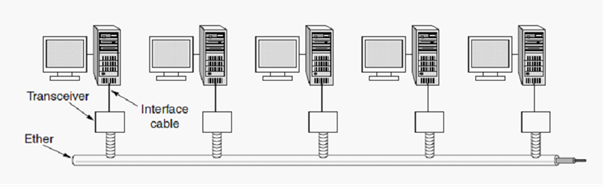
\includegraphics[scale = 0.5]{assets/jisuanjiwangluo_b6529.png}
  \caption{经典以太网}
\end{figure}

\begin{figure}[H]
  \centering
  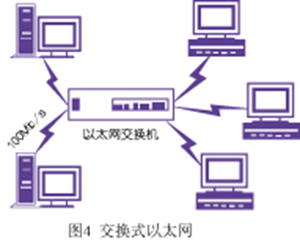
\includegraphics[scale = 0.5]{assets/jisuanjiwangluo_c2575.png}
  \caption{交换式以太网}
\end{figure}

\begin{figure}[H]
  \centering
  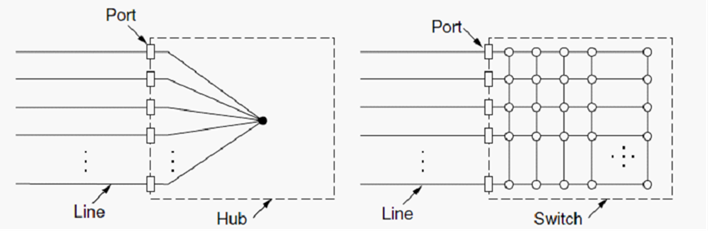
\includegraphics[scale = 0.5]{assets/jisuanjiwangluo_99ba0.png}
  \caption{集线器与交换机的区别}
\end{figure}

\spaceline
\textbf{以太网的命名规则:}
\begin{figure}[H]
  \centering
  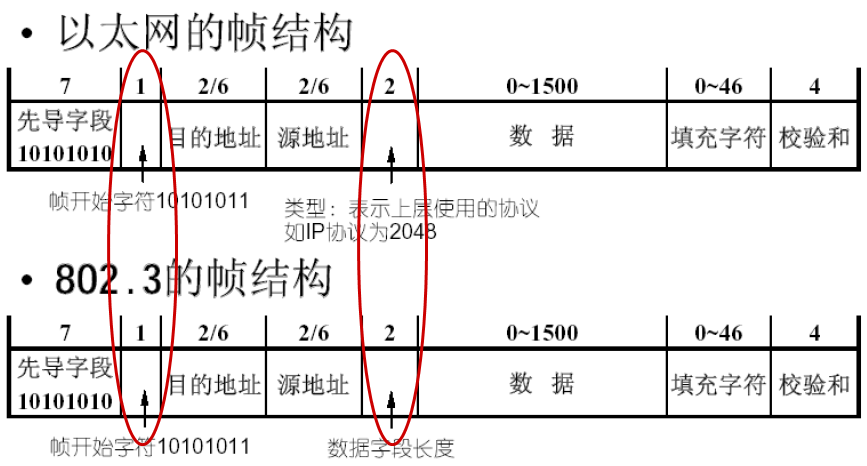
\includegraphics[scale = 0.5]{assets/jisuanjiwangluo_7de21.png}
  \caption{以太网的命名规则,分段长度中,2表示200米的意思,基本单位是100米}
\end{figure}

\spaceline
\textbf{以太网的编码方式:}采用曼彻斯特编码
对于802.5采用差分曼彻斯特协议

\spaceline
\textbf{IEEE802.3与以太网帧组成的区别:}
\begin{figure}[H]
  \centering
  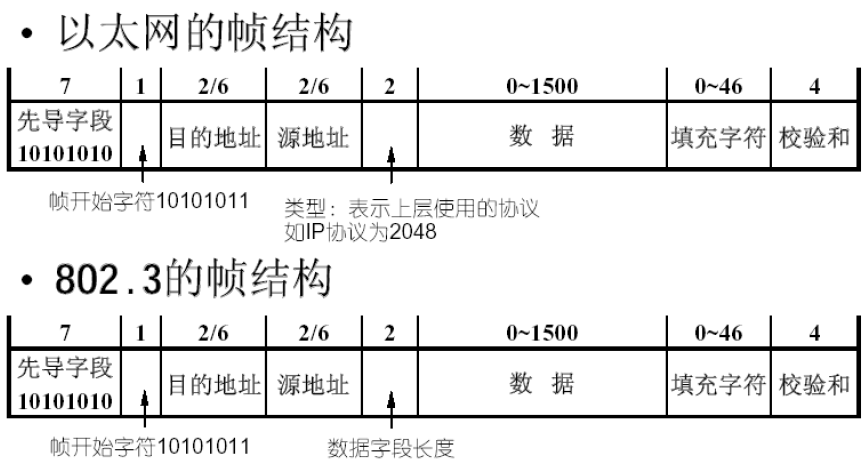
\includegraphics[scale = 0.3]{assets/jisuanjiwangluo_f7e24.png}
  \caption{IEEE802.3与以太网帧组成的区别}
\end{figure}

\spaceline
\textbf{802.3的帧组成:}
\begin{figure}[H]
  \centering
  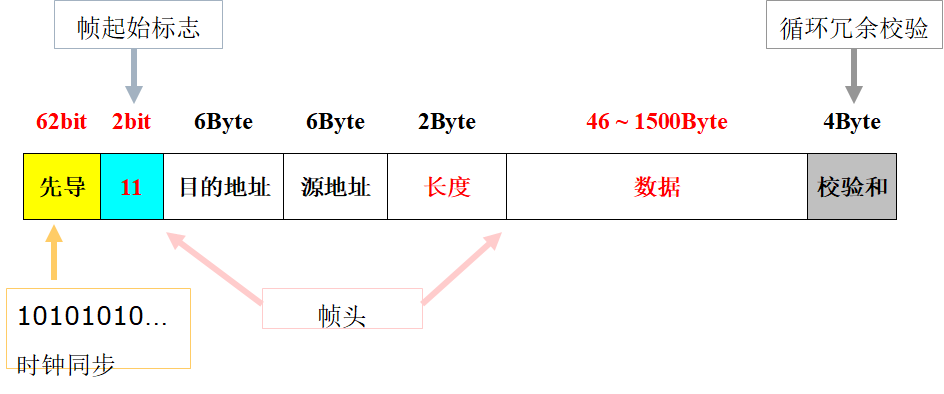
\includegraphics[scale = 0.4]{assets/jisuanjiwangluo_e1f57.png}
  \caption{802.3的帧组成}
\end{figure}

\textbf{最短帧长:}64B
\begin{itemize}
  \item 帧头\\
  6B目的地址,6B源地址,2B长度
  \item 数据位\\
  最少46B
  \item 校验位\\
  4B
\end{itemize}
{\color{blue}貌似没有计算先导字段}

\spaceline
\textbf{MAC地址:}物理地址,xx:xx:xx:xx:xx:xx
\begin{figure}[H]
  \centering
  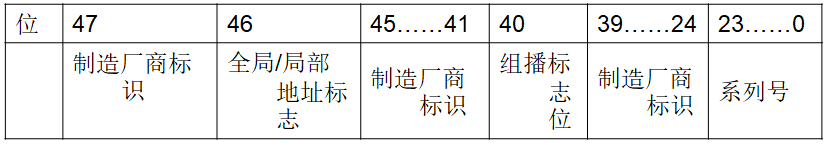
\includegraphics[scale = 0.3]{assets/jisuanjiwangluo_1fa17.png}
  \caption{MAC地址组成:前24位表示公司}
\end{figure}

\spaceline
\textbf{长度字段:}帧最短长度为64B,最大为1518B

{\color{red}为什么是64B?为什么是1518B?为什么要有最短长度?P227,第一问在后面有解答}

\spaceline
\textbf{数据字段:}最少为64B,不够则填充

\spaceline
\textbf{帧校验字段:}采用32b,CRC校验

\textbf{怎么区分到底代表类型型还是长度呢}
检查这个字段的数值:如果小于等于 1536(0x600),则是长度(802.3)字段,如果大于 1536,则表示类型(以太帧)

\textbf{为什么要大于64B?}
\begin{figure}[H]
  \centering
  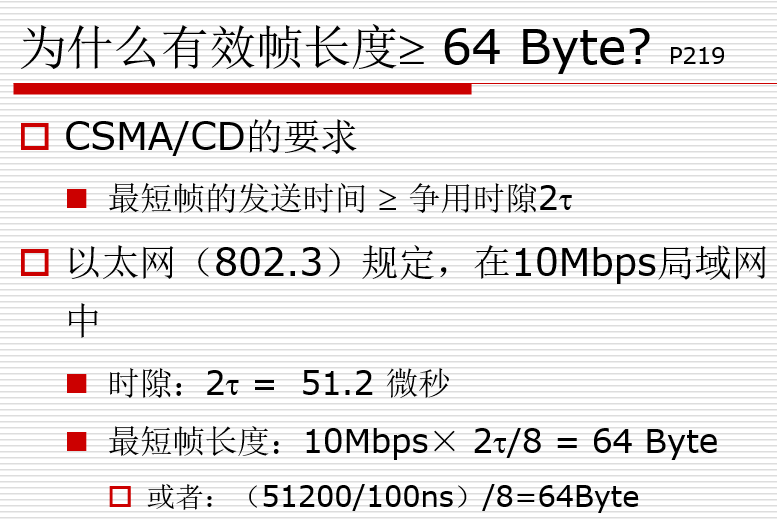
\includegraphics[scale = 0.3]{assets/jisuanjiwangluo_02c3a.png}
  \caption{为什么要大于64B?}
\end{figure}

{\color{red}为什么要51.2微秒的时隙?}

\spaceline
\textbf{二进制指数后退法:}有冲突检测的载波侦听策略当冲突的时候会随机等待一段时间,那么这个时间的范围什么确定?\\
\begin{figure}[H]
  \centering
  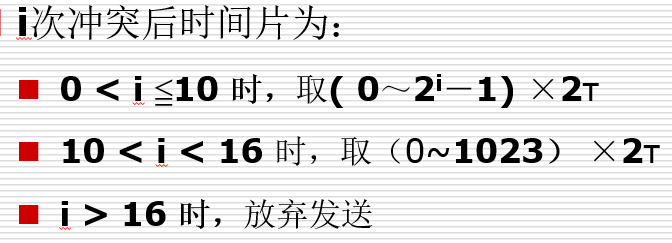
\includegraphics[scale = 0.3]{assets/jisuanjiwangluo_d029d.png}
  \caption{第i次冲突等待时间}
\end{figure}

进一步优化:一般确认接收之后,则下一个时隙留给接收方返回确认消息,而不是进入新的一轮竞争

\subsection{快速以太网(100M)}
以太网提高负载的方法:
\begin{itemize}
  \item 提速到100M
  \item 全双工
  \item 使用交换机代替集线器
\end{itemize}

100M以太网:保留原来的帧格式、接口和偶成UI则,只是将比特时间从100ns降低到10ns(物理上表现为电缆长度为原来的$\frac{1}{10}$)

\begin{figure}[H]
  \centering
  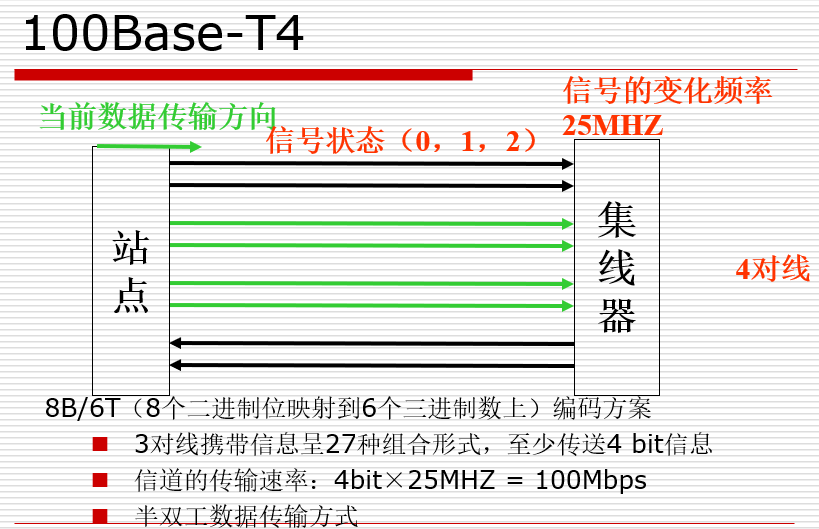
\includegraphics[scale = 0.3]{assets/jisuanjiwangluo_7150c.png}
  \caption{100BaseT4}
\end{figure}


\begin{figure}[H]
  \centering
  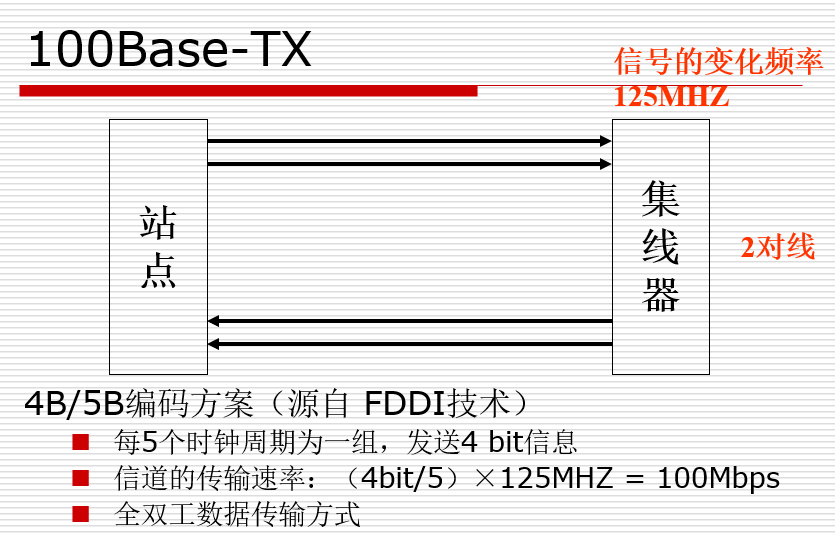
\includegraphics[scale = 0.3]{assets/jisuanjiwangluo_7fbf4.png}
  \caption{100BaseTX}
\end{figure}


\section{交换机}
\textbf{网桥与交换机的关系:}就像中继器与集线器的关系

\subsection{千兆以太网(1000M)}
出现的问题:1000M以太网速度太快导致传输时间太短,进而传输的距离也短
\begin{figure}[H]
  \centering
  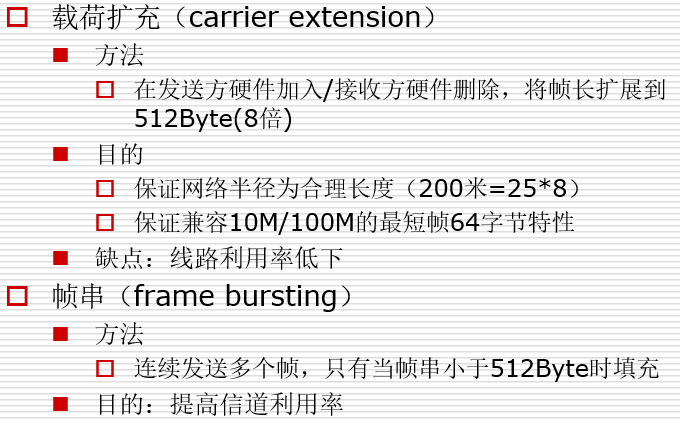
\includegraphics[scale = 0.5]{assets/jisuanjiwangluo_72a2b.png}
  \caption{千兆以太网解决办法}
\end{figure}

注:计算机网络中一般取$1M = 10^6 , 1K = 10^3$,存储单位采取2的指数
\end{document}
